\documentclass[tikz,border=2pt]{standalone}
\usepackage{unicode-math}
\setmainfont[
  Path=publication/fonts/,
  UprightFont=source-serif-4-latin-400-normal.ttf,
  ItalicFont=source-serif-4-latin-400-italic.ttf,
  BoldFont=source-serif-4-latin-600-normal.ttf,
  BoldItalicFont=source-serif-4-latin-600-italic.ttf
]{Source Serif 4}
\setmathfont[Path=/System/Library/Fonts/Supplemental/]{STIXTwoMath.otf}
\usepackage{tikz}
\usetikzlibrary{arrows.meta,backgrounds,calc,decorations.pathreplacing,fit,matrix,positioning}
\definecolor{BookInk}{HTML}{18232D}
\definecolor{BookBlue}{HTML}{315F78}
\definecolor{BookRed}{HTML}{98452F}
\definecolor{BookGreen}{HTML}{3F6659}
\definecolor{BookMuted}{HTML}{66727A}
\definecolor{BookRule}{HTML}{AEB7BC}
\tikzset{
  book/node/.style={
    draw=BookInk, line width=.55pt, fill=white,
    minimum height=9mm, inner xsep=5pt, inner ysep=4pt,
    font=\footnotesize, align=center
  },
  book/primary/.style={book/node, draw=BookBlue},
  book/decision/.style={book/node, draw=BookRed},
  book/verified/.style={book/node, draw=BookGreen},
  book/arrow/.style={
    -{Stealth[length=2mm,width=1.35mm]}, line width=.55pt, draw=BookInk
  },
  book/quietarrow/.style={
    -{Stealth[length=2mm,width=1.35mm]}, line width=.45pt, draw=BookRule
  },
  book/feedback/.style={
    -{Stealth[length=2mm,width=1.35mm]}, line width=.5pt,
    draw=BookRed, dashed
  },
  book/note/.style={font=\scriptsize, text=BookMuted, align=center}
}

\begin{document}
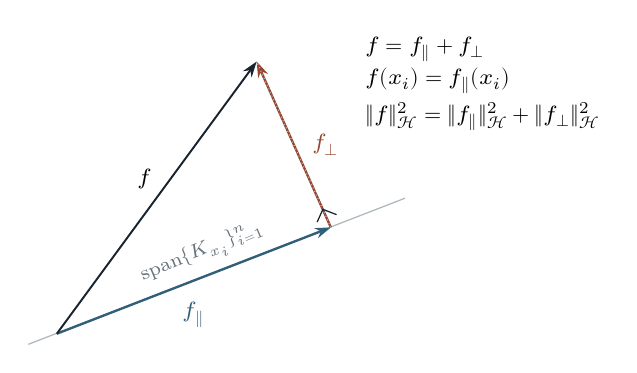
\begin{tikzpicture}[x=1.45cm,y=1.35cm,every node/.append style={font=\footnotesize}]
  \coordinate (o) at (0,0);
  \coordinate (p) at (2.4,1);
  \coordinate (f) at (1.75,2.56);
  \draw[BookRule,line width=.45pt] (-.25,-.1) -- (3.05,1.275);
  \node[book/note,rotate=22.6,anchor=south] at (1.35,.57)
    {$\operatorname{span}\{K_{x_i}\}_{i=1}^{n}$};
  \draw[book/arrow,draw=BookBlue,line width=.85pt] (o) -- (p)
    node[midway,below=4pt,text=BookBlue] {$f_{\parallel}$};
  \draw[book/arrow,draw=BookRed,line width=.85pt] (p) -- (f)
    node[midway,right=3pt,text=BookRed] {$f_{\perp}$};
  \draw[book/arrow,line width=.7pt] (o) -- (f)
    node[pos=.57,left=4pt] {$f$};
  \draw[BookRule,densely dotted] (p) -- (f);
  \draw[BookInk,line width=.45pt] ($(p)+(-.12,.05)$) -- ($(p)+(-.07,.17)$)
    -- ($(p)+(.05,.12)$);
  \node[anchor=west,align=left] at (2.62,2.35)
    {$f=f_{\parallel}+f_{\perp}$\\[2pt]
     $f(x_i)=f_{\parallel}(x_i)$\\[2pt]
     $\|f\|_{\mathcal H}^{2}
       =\|f_{\parallel}\|_{\mathcal H}^{2}+\|f_{\perp}\|_{\mathcal H}^{2}$};
\end{tikzpicture}
\end{document}
